
%----------------------------------------------------------------------------------------
%	PACKAGES AND DOCUMENT CONFIGURATIONS
%----------------------------------------------------------------------------------------

\documentclass[a4paper]{article} %Article class
\usepackage[utf8]{inputenc} %utf-8 Encoding
\usepackage{graphicx} % Required for the inclusion of images
\usepackage{float} %requiered for image positioning
\graphicspath{{Figures/}} % Set the default folder for images
\usepackage{amsmath} % Required for some math elements 
\usepackage[catalan]{babel} % Language 
\setlength\parindent{0pt} % Removes all indentation from paragraphs
\usepackage{xcolor}	
\usepackage{listings} %Requiered for code inclusion
\renewcommand{\labelenumi}{\alph{enumi}.} % Make numbering in the enumerate environment by letter rather than number (e.g. section 6)
\usepackage[
backend=biber,
style=numeric,
sorting=ynt
]{biblatex}
\addbibresource{sample.bib}

\usepackage{color}
\lstset{ %
	language=R,                     % the language of the code
	basicstyle=\footnotesize,       % the size of the fonts that are used for the code
	numbers=left,                   % where to put the line-numbers
	numberstyle=\tiny\color{gray},  % the style that is used for the line-numbers
	stepnumber=1,                   % the step between two line-numbers. If it's 1, each line
	% will be numbered
	numbersep=5pt,                  % how far the line-numbers are from the code
	backgroundcolor=\color{white},  % choose the background color. You must add \usepackage{color}
	showspaces=false,               % show spaces adding particular underscores
	showstringspaces=false,         % underline spaces within strings
	showtabs=false,                 % show tabs within strings adding particular underscores
	frame=single,                   % adds a frame around the code
	rulecolor=\color{black},        % if not set, the frame-color may be changed on line-breaks within not-black text (e.g. commens (green here))
	tabsize=2,                      % sets default tabsize to 2 spaces
	captionpos=b,                   % sets the caption-position to bottom
	breaklines=true,                % sets automatic line breaking
	breakatwhitespace=false,        % sets if automatic breaks should only happen at whitespace
	title=\lstname,                 % show the filename of files included with \lstinputlisting;
	% also try caption instead of title
	keywordstyle=\color{blue},      % keyword style
	commentstyle=\color{dkgreen},   % comment style
	stringstyle=\color{mauve},      % string literal style
	escapeinside={\%*}{*)},         % if you want to add a comment within your code
	morekeywords={*,...},
	% if you want to add more keywords to the set
	alsoletter={.}        % if you want to add more keywords to the set
} 


%----------------------------------------------------------------------------------------
%	DOCUMENT INFORMATION
%----------------------------------------------------------------------------------------

\title{Network Intruder Detection \\
\large Pràctica APA \\
Universitat Politècnica de Catalunya} % Title
\author{Lluc Bové \& Aleix Trasserra} % Author name

\date{Q1 2016-17}

\begin{document}

\maketitle % Insert the title, author and date
\newpage
\tableofcontents
\newpage
%----------------------------------------------------------------------------------------
%	INTRO
%----------------------------------------------------------------------------------------

\section{Introducció}
En l'àrea de la \textit{seguretat informàtica}, una de les principals àrees d'investigació actual és la de protegir les xarxes dels usuaris no autoritzats.
Un problema rellevant és predir si una connexió és un atac a la seguretat del sistema (i quin tipus d'atac) o bé si es tracta d'una connexió normal d'un usuari autoritzat.
L'objectiu d'aquest document és explicar els diversos mètodes que hem usat per poder classificar automàticament els atacs descrits. Començarem per un context sobre el problema, descriurem les dades i explicarem el procés de preprocessat que hem dut a terme, les visualitzarem, explicarem els resultats de diversos mètodes provats de classificació, primer lineals i després no lineals, justificarem quin mètode hem escollit(xarxes MLP) i el seu error de generalització i per últim explicarem les conclusions obtingudes.

\subsection{Les dades}
Les nostres dades\cite{kdd} són un conjunt de files on cada fila és una \textbf{connexió}.
Una \textbf{connexió} és un conjunt de paquets TCP començant i acabant en uns períodes de temps coneguts. Les dades d'aquest conjunt de paquets es transporten des d'una adreça IP origen fins a una altra adreça IP destí sota un determinat \textit{protocol}. \\
Hi ha quatre tipus d'atacs diferents que el sistema ha de ser capaç d'identificar a banda de les connexions que no són atacs. Aquestes són:
\begin{itemize}
	\item DOS: denegació de servei.
	\item R2L: accés no autoritzat des d'una màquina remota.
	\item U2R: accés no autoritzat a privilegis de "root" (superuser).
	\item probing: vigilància i altres tipus de  "probing", per exemple: port scanning.
\end{itemize}




%----------------------------------------------------------------------------------------
%	Related
%----------------------------------------------------------------------------------------

\section{Treballs relacionats}
Hem trobat varis treballs relacionats. El primer\cite{JAM} descriu els resultats obtinguts utilitzant un sistema distribuït basat en \textit{Data Mining} anomenat JAM que té per objectiu abordar el problema de detecció d'intrusos en sistemes d'informació financers.
Un altre investigació relacionada amb la \textit{detecció de connexions fraudulentes}\cite{PNRule} parla sobre un \textit{framework} basat en un tipus de regles anomenades \textbf{PN-rule}. Aquest permet obtenir models de classificació i va utilitzar la detecció de connexions fraudulentes per experimentar.

A més també hi ha un article d'un dels participants del concurs \textit{kdd} on s'havia de resoldre el mateix problema\cite{kdd3}. En aquest cas l'equip participant anomenat \textit{MP3} utilitzava un mètode basat en un conjunt d'arbres de decisió, on es decidia per votació.
%----------------------------------------------------------------------------------------
%	Data exploration
%----------------------------------------------------------------------------------------

\section{Exploració de dades}

L'objectiu d'aquesta secció és fer un primer cop d'ull a les nostres dades per tal de tenir una visió més clara sobre com són les dades que haurem d'analitzar posteriorment.
El primer pas  és fer un \textit{pre-processat} de les dades. Aquest pas inclou detectar possibles \textit{outliers}, identificar si existeixen \textit{missing values} i si és el cas, eliminar-los.
Seguidament realitzarem \textit{feature extraction and selection} que consisteix a esborrar variables que no aporten informació i/o obtenir noves variables a partir de les ja existents que ens aportin nova informació sobre com són les nostres dades. Per últim visualitzarem les nostres dades usant \textit{FDA} seguit d'un procés de \textit{clustering}. El procés descrit es pot seguir utilitzant l'\textit{script} proveït anomenat \textit{dataExploration.R}.


\subsection{Preprocessat}

Les dades originals se'ns han proveït de dues formes: la primera conté aproximadament unes 5 milions de connexions mentre que l'altra conté un 10\% de les dades originals aproximadament.

El primer que veiem quan analitzem les dades,és que hi ha variables sense nombrar, per tant les hem nombrat. Seguidament executem \lstinline|summary| amb la finalitat de detectar anomalies de les dades com ara mitjanes o medianes estranyes, valors extrems, errors etc. Hem vist que hi ha variables categòriques que apareixen en forma d'enters. Les que són booleanes les hem transformat amb els factors \lstinline|TRUE| i \lstinline|FALSE| i per la resta hem utilitzat text(noms que les identifiquen els factors). També hem observat variables que sempre tenen el mateix valor i les hem eliminat. Hem detectat que hi havien \textit{missing values} en una variable booleana i el que hem fet és eliminar les files que tenien el problema esmentat.


\subsection{Feature extraction/selection}

El primer que hem de fer és definit una variable resposta. Hem decidit utilitzar com a tal la variable \textit{main\_attack}.
Aquesta defineix una categoria per a cada tipus d'atac. La definició de la variable es pot veure a la taula \ref{table:main}:

\begin{table}
	\begin{tabular}{ll}
		Main Attack & Tipus d'atac                                                            \\ \hline
		DOS         & back, land, neptune, smurf, teardrop                                       \\
		U2R         & buffer overflow, loadmodule, perl, rootkit                               \\
		R2L         & ftp\_write, guess password, imap, multihop,\\ & phf, spy, warezclient, warezmaster \\
		probe       & ipsweep, nmap, portsweep, satan                                           \\
		normal      & normal                                                                 \\
	\end{tabular}
	\caption{Aquesta taula mostra la classificació de la variable \textit{main\_attack}}
	\label{table:main}
	
\end{table}



\subsection{Anàlisi Estadística Descriptiva}
Procedim a realitzar un anàlisi de l'estadística descriptiva de les nostres dades. Usem el paquet \textit{ggplot2}\cite{ggplot} per fer les nostres gràfiques més boniques. Per a totes les variables numèriques mostrem un histograma i un \textit{boxplot}. Ens adonem que hi ha moltes variables amb mediana 0, ja que hi ha moltes observacions amb valor 0 i això fa que la mediana se situï al 0 ja que com a mínim la meitat de les observacions són 0. Això és perquè hi ha molts camps de TCP com els bytes enviats (molts cops no s'envien dades) que en molts casos no s'usa i per això està a zero. Així que és important si la comunicació és entre el host i el servidor o viceversa. Apliquem logaritmes a les variables que ho puguin necessitar però per veure'n l'efecte d'algunes variables excloem les observacions amb valor zero ja que són moltes i distorsionen la gràfica. Mostrem alguns d'aquests gràfics.

\begin{figure}[H]
	\centering
	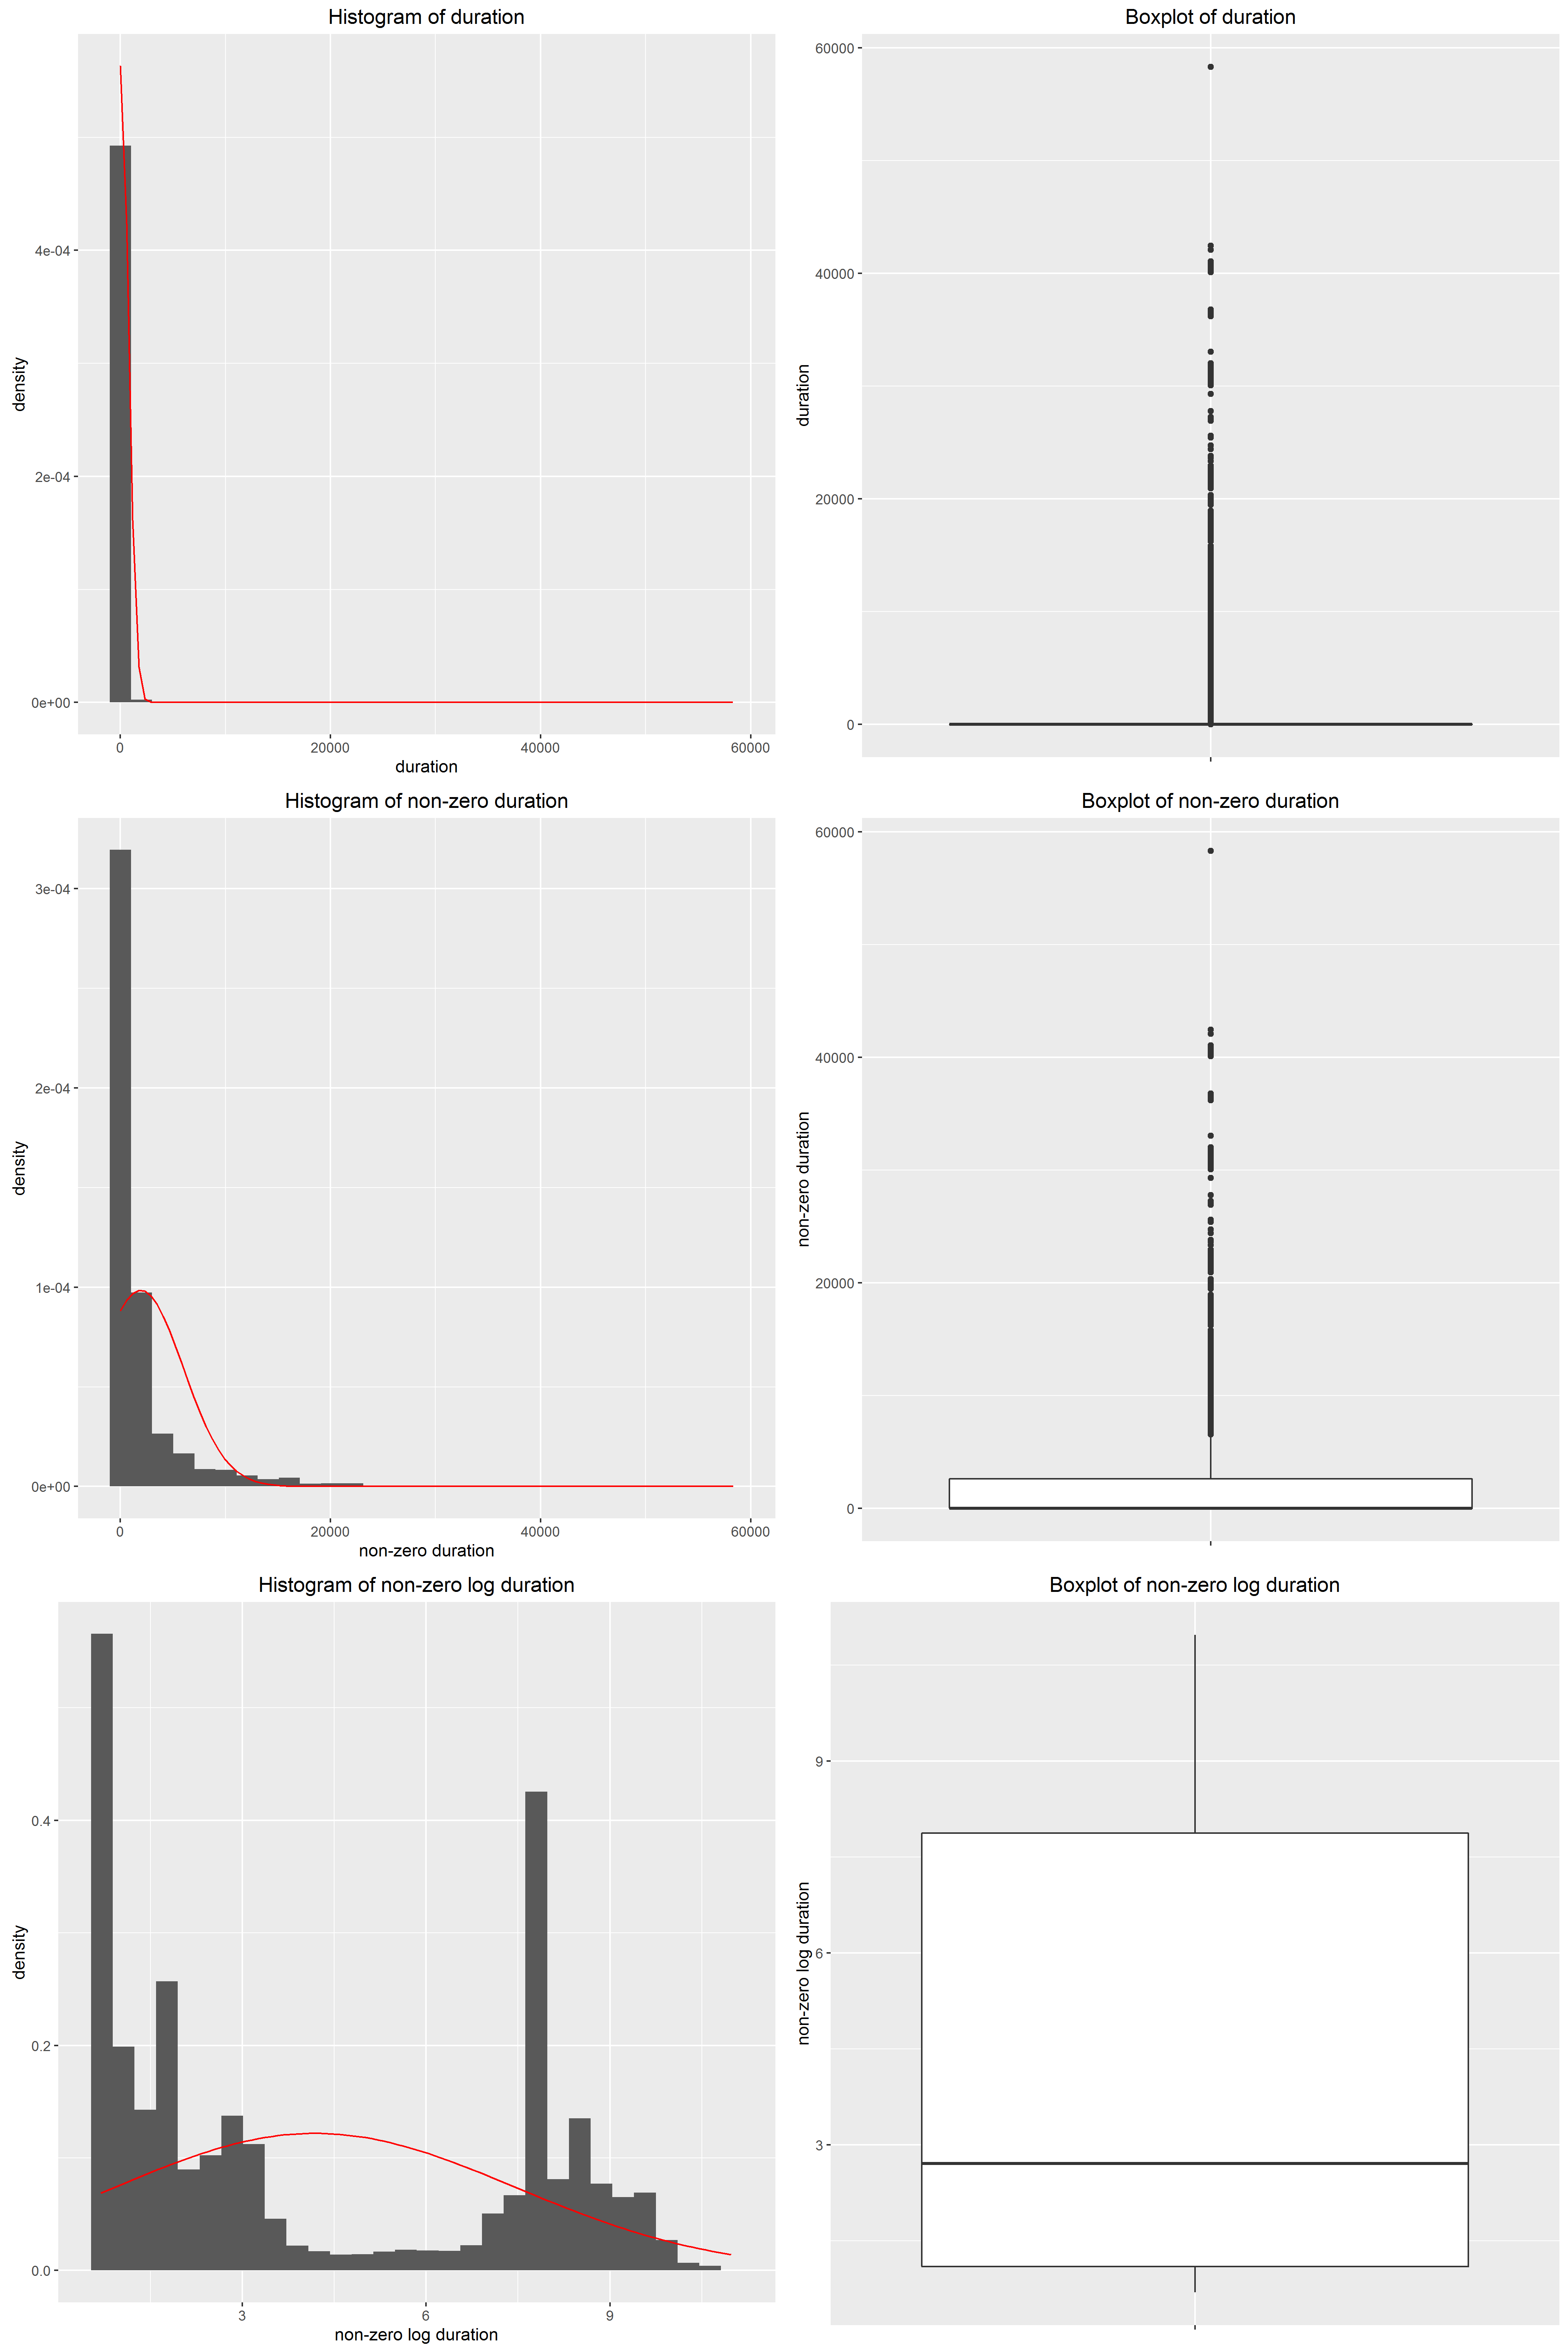
\includegraphics[scale=0.25]{duration.png}
	\caption{Gràfiques descriptives per la variable duració}
	\label{fig:duration}
\end{figure}

La figura \ref{fig:duration} mostra el \textit{boxplot} i l'histograma de la variable \textit{duration}, que descriu la duració de la connexió TCP. Podem observar que la majoria de connexions duren menys d'un segon i per tant es marquen com a zero. Això fa que tinguem problemes per visualitzar els gràfics. Per això si no incloem els valors amb zero podem observar-ho millor. Aquesta variable és millor si apliquem una transformació logarítmica.
Moltes variables tenen la mateixa estructura que duració així que no les influïm a la documentació. A continuació descriurem les variables categòriques. Per a fer-ho utilitzem taules de contingència i gràfics de barres.

La figura \ref{fig:barplots} mostra un gràfic de barres per la variable que volem predir, \textit{main\_attack}. Emfatitzem el fet de que té una distribució molt poc equilibrada. La majoria d'observacions són atacs DOS i segueixen les connexions normals. \textit{Probe} ja està amb molt poca proporció respecte les altres i gairebé no hi ha observacions de \textit{R2L} ni de \textit{U2R}. Més endavant explicarem com hem abordat aquest problema.

\begin{figure}[H]
	\centering
	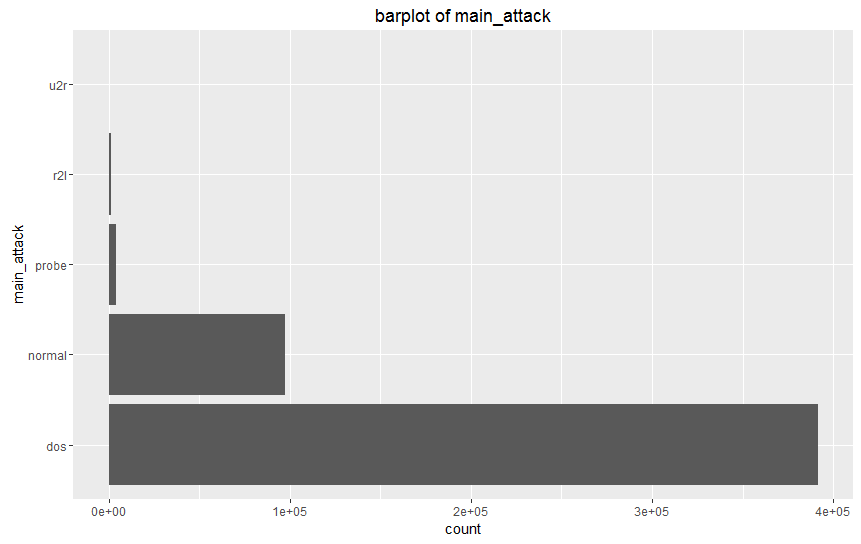
\includegraphics[scale=0.5]{bar_main_attack.png}
	\caption{Gràfic de barres de \textit{main\_attack}}
	\label{fig:barplots}
\end{figure}
Mostrem taules de contingència de les variables categòriques més rellevants, respecte la variable que predim, \textit{main\_attack}. Aquestes són \textit{protocol}, \textit{flags}, \textit{service} i \textit{superuser attempted}. La figura \ref{fig:cont} mostra el resultat.

\begin{figure}[H]
	\centering
	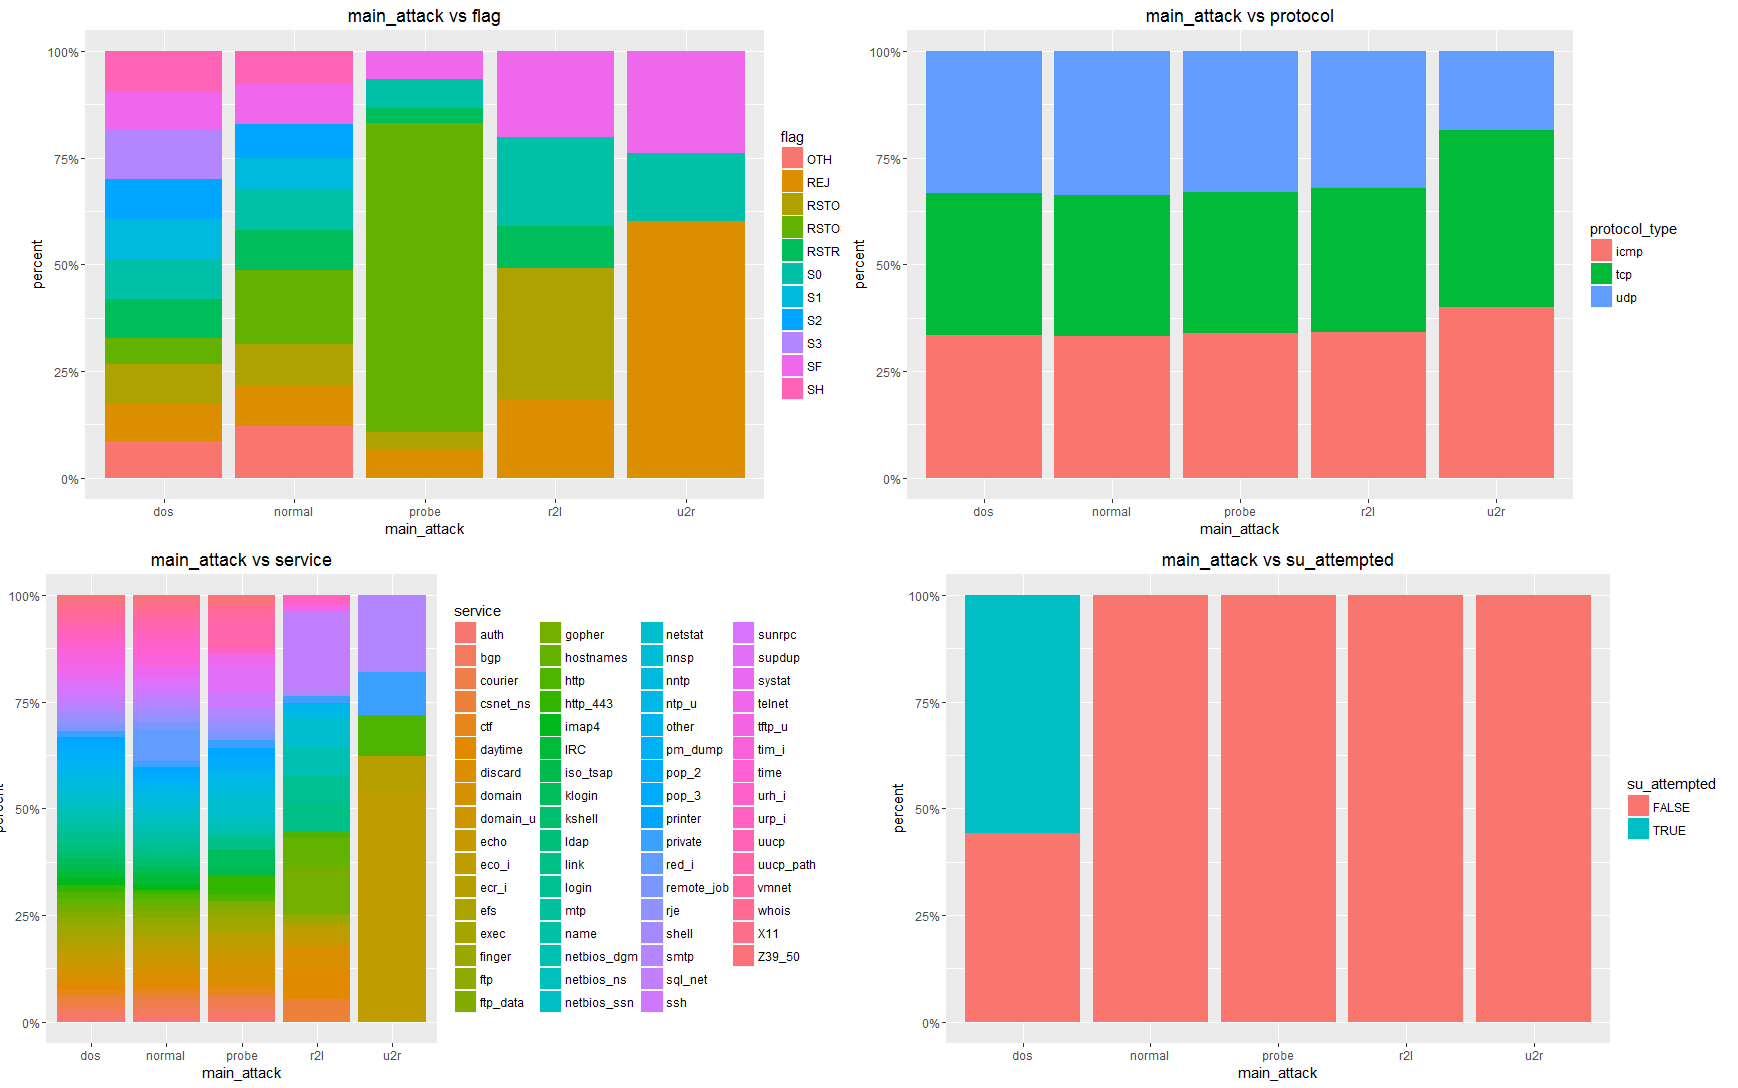
\includegraphics[scale=0.85]{cont.png}
	\caption{Taules de contingència de les variables més rellevants respecte la variable resposta, representades com a gràfics de barres. }
	\label{fig:cont}
\end{figure}

Podem observar que per exemple, els atacs DOS i les connexions normals tenen flags similars, als atacs probe el flag \textit{RESET} és molt comú, i a \textit{U2R} predomina el flag \textit{REJ}. Pel que fa els protocols tots els tipus d'atacs n'utilitzen de similars. Els serveis usats són molt similars amb les connexions normals, i els atacs DOS i probe. Difereixen amb els atacs R2L i U2L i el servei que predomina en U2R és \textit{eco\_i}. L'únic atac que demana permisos d'administrador és l'atac DOS.

Finalment, per poder solucionar el problema de les dades que no estan balancejades utilitzem bàsicament dues tècniques:
\begin{itemize}
    \item Eliminar instàncies de les classes amb més observacions
    \item Crear observacions artificials de les classes amb menys observacions.
\end{itemize}
Així doncs obtenim un nou \textit{dataset} aplicant aquestes tècniques. Per aplicar la primera eliminem instàncies de forma aleatòria i uniforme. Per aplicar la segona tècnica usem \textit{SMOTE}\cite{SMOTE}, implementat pel paquet d'R \textit{DMwR}\cite{DMwR}. Usarem doncs els dos \textit{datasets} per realitzar els diferents experiments.

\subsection{Visualització}
Per poder visualitzar les dades usem L'Anàlisi Discriminant de Fisher o FDA. L'apliquem només amb les variables numèriques i usant com a classe la variable que volem predir. També visualitzarem els dos conjunts de dades que hem generat, el complet i el balancejat. Comencem per les dades completes. La visualització de les dues primeres components es pot veure a la figura \ref{fig:fda}.

\begin{figure}[H]
	\centering
	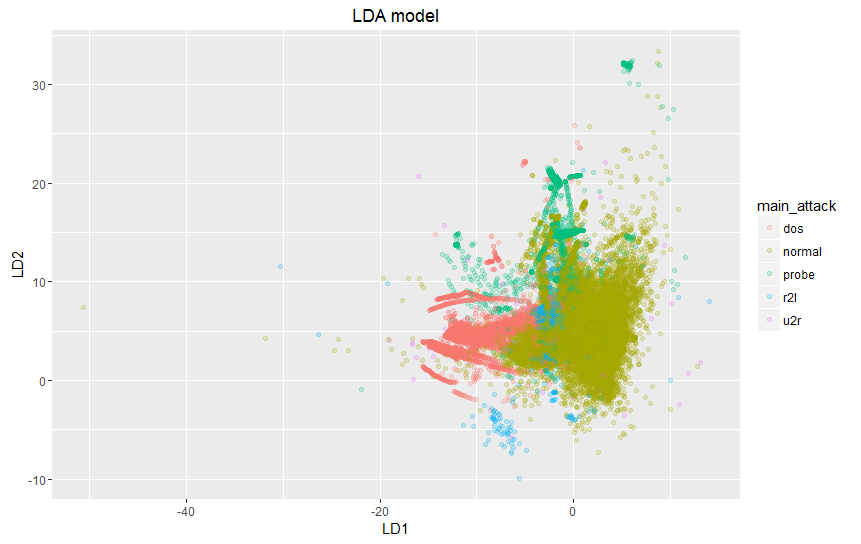
\includegraphics[scale=0.45]{LDA.png}
	\caption{Visualització amb FDA del conjunt de dades complet}
	\label{fig:fda}
\end{figure}

Les classes no es veuen especialment separades, de fet si no utilitzéssim colors probablement no sabríem distingir quina classe és quina. Això ens indica que possiblement la tasca de classificació serà complexa. La suma dels dos primers components suma un 98.49\%, així que realment una tercera component no aportaria molta variància. La figura \ref{fig:fda_bal} mostra les dues primeres components de l'anàlisi FDA per el conjunt de dades balancejades. Es pot veure que aquí les classes estan més separades que abans, tot i que n'hi ha molt menys volum. Tot i això es pot veure bastant sol·lapament entre classes i moltes observacions que estan a les fronteres entre el que podria ser una hipotètica separació entre classes.

\begin{figure}[H]
	\centering
	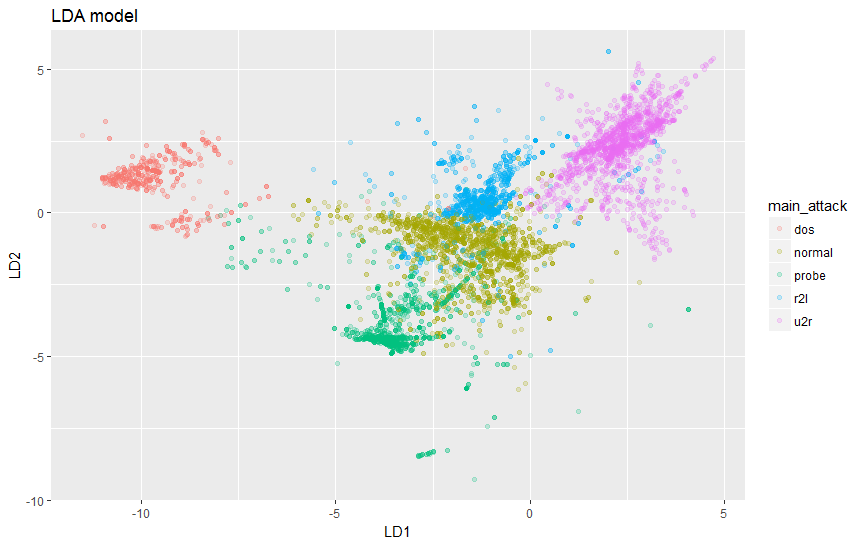
\includegraphics[scale=0.45]{lda_balanced.png}
	\caption{Visualització amb FDA del conjunt de dades balancejat}
	\label{fig:fda_bal}
\end{figure}

\subsection{Clustering}
En aquesta secció explicarem els resultats obtinguts en el procés de "clustering".
L'objectiu d'aquest procés és identificar el nombre de "clusters" que explica millor com són les nostres dades i també veure quina n'és la seva agrupació.
La nostra intuïció ens diu que el nombre de grups de dades hauria de ser igual a 5 (un per cada tipus d'atac).
Hem aplicat l'algorisme de \textit{k-means} ja que funciona força bé i el temps computacional no és prohibitiu.

Hem dut a terme un experiment que consisteix a executar l'algorisme 50 vegades per cadascun dels nombre de clusters entre 2 i 11 i hem agafat la mitjana del nombre d'execucions. L'objectiu de l'experiment és determinar quin és el nombre de clusters i el fet de repetir l'execució vàries vegades té com a finalitat minimitzar possibles valors anòmals derivats de l'aleatorietat de \textit{k-means}.

\begin{figure}[H]
	\centering
	\includegraphics[scale=0.45]{clustering.png}
	\caption{Nombre de clusters vs C-H índex}
	\label{fig:clust}
\end{figure}

A la figura \ref{fig:clust} podem veure l'evolució de l'índex de \textit{Calinski-Harabasz} a mesura que anem augmentant el nombre de clusters. Com es pot observar, quan el nombre de clusters és entre 4 i 7 és quan l'índex és mes elevat, fet que indica que la qualitat d'aquests és més elevada. Aquest fet concorda amb la intuïció inicial. La variació que es veu pot ser deguda a que hi ha subclasses d'atacs.



%----------------------------------------------------------------------------------------
%	Classification
%----------------------------------------------------------------------------------------

\section{Classificació}
\subsection{Mètodes Lineals}
\subsubsection{Regressió logística}
En aquesta secció mostrarem els resultats obtinguts al usar regressió logística.
La regressió logística només funciona per classes binàries i la nostra classe no ho és, així doncs mirarem de predir les connexions com a \textit{connexió normal} o com a \textit{atac}.

Primer de tot entrenem el nostre model usant la \textit{logistic regression} amb totes les dades, que sabem que no són equilibrades.
Usem l'índex AIC \cite{wiki:AIC} per simplificar el model.
Denotem \textit{P} com al punt de tall de la regressió logística.
Usem \textit{P} tenint en compte que preferim que es predigui una connexió normal com a atac(fals positiu) que no que un atac es predigui com a connexió normal(fals negatiu) ja que passaria inadvertit i podria tenir conseqüències greus.
Hem provat valors de  P dins del rang $(0.4,0.7)$ en passos de $0.1$.
\begin{table}[h]
	\centering
	\begin{tabular}{l|llll}
		P              & 0.4  & 0.5   & 0.6   & 0.7   \\
		\hline 
		Training error & 30.4 & 30.46 & 30.54 & 30.63 \\
		Test error     & 7.67 & 7.71  & 7.75  & 7.79 
	\end{tabular}
	\caption{Errors d'entrenament i de test de regressió logística depenent de P}
	\label{cut}
\end{table}

Si observem la taula \ref{cut}, per P=0.4 obtenim els errors més baixos. 
S'ha de dir que no només hem observat els valors dels errors sinó també les matrius de confusió per poder veure que es compleixi que hi hagi menys falsos negatius que falsos positius.
Observem doncs la matriu de confusió amb $P = 0.4$ que mostra la taula \ref{logistic}. Podem observar que el ràtio de falsos positius és del 9.10\% i el de positius verdaders del 1.75\%  . 

\begin{table}[h]
	\centering
	\begin{tabular}{l|ll}
		& Pred   &        \\
		Truth  &        &        \\
		& normal & attack \\
		\hline
		normal & 59526  & 1063   \\
		attack & 22790  & 227646
	\end{tabular}
	\caption{Matriu de confussió de la regressió logística amb P = 0.4}
	\label{logistic}
\end{table}


\subsubsection{Multinomial regression}
Hem decidit també provar d'usar una regressió multinomial. Coneixem que les dades són no balancejades però primer provem les dades sense tractar. Obtenim un error de train del 0.05\%, i un de test de 7.79\%,. Malgrat l'error de test sigui baix, les classes minoritàries com \textit{U2R} o \textit{R2L} es generalitzen molt malament, tal i com la taula \ref{table:unbModel} mostra. Un alt percentatge d'atacs \textit{U2R} es prediuen malament,i són els més perillosos de detectar. A més a més es moltes observacions que són d'aquest atac es prediuen com a connexions normals i per tant passaran totalment inadvertides. 

\begin{table}[H]
	\centering
	\begin{tabular}{c | c c c c c}
		& Prediction\\
		Truth\\
		 & Normal & DOS & Probe & R2L & U2R \\
		\hline
		Normal	& 59511	& 95 	 & 953	 & 16 	& 14 \\
		DOS		& 5925	& 223563 & 135	 & 0  	& 807\\
		Probe	& 625	& 163	 & 3125	 & 253	& 0 \\
		R2L		& 15588	& 0		 & 8   & 568 	& 25\\
		U2R		& 190	& 0		 & 0    & 11 	& 27\\	
	\end{tabular}
	\caption{Taula de contingència del model multinomial que usa totes les dades}
	\label{table:unbModel}
\end{table}


Per solucionar el problema de tenir les dades no balancejades usem les dades que hem balancejat. Apliquem regularització i trobem la constant $\lambda$ amb 10-cross-validation. Usem el paquet de \textit{R} \textit{glmnet} \cite{glmnet} que implementa la regularització. L'error d'entrenament és del 1.3\% i el de test és del 7.88\%.


\begin{table}[H]
	\centering
	\begin{tabular}{c | c c c c c}
			& Prediction\\
		Truth\\
				& Normal & DOS & Probe & R2L & U2R \\
		\hline
		Normal	& 58443	& 685 	 & 457	 & 503 	& 503 \\
		DOS		& 5623	& 223376 & 359	 & 38  	& 457\\
		Probe	& 518	& 38	 & 3538	 & 69	&  3 \\
		R2L		& 14611	& 1		 & 193   & 1107 & 277\\
		U2R		& 44	& 6		 & 123    &  7 	& 48\\	
	\end{tabular}
	\caption{Taula de contingència per el model multinomial amb dades balancejades i reduït usant regularització}
	\label{table:sub10model}
\end{table}

La taula \ref{table:sub10model} mostra la taula de contingència del model. Les columnes mostren la predicció i les files el valor real. Es mostra la taula per les dades de test així que és una mostra de com generalitza el model. Malgrat l'error de test sigui pitjor que el model entrenat amb el conjunt de dades balancejat, les prediccions de les classes minoritàries són més precises, en general. Per exemple en el cas de \textit{U2R} reduïm el nombre d'atacs que són predits com a connexions normals i augmentem el nombre d'atacs predits correctament a gairebé el doble. El mateix passa amb els atacs \textit{R2L} i en menys mesura amb els atacs \textit{probe}.

\subsubsection{LDA}
Finalment l'últim dels mètodes lineals que hem provat ha estat LDA. Aquest mètode té la restricció que només es pot usar amb dades numèriques. Hem provat utilitzant el conjunt de dades sencer com també el balancejat. En aquest cas el balancejat ha donat pitjors resultats, on tant l'error d'entrenament i de test són pitjors i està menys equilibrat que l'altre en el sentit que prediu pitjor les classes més minoritàries. Així doncs amb el model fent servir el conjunt de dades sencer obtenim un error d'entrenament del 0.93\% i un de test del 7.48\% en contrast del  4.86\% i 8.26\% que obtenim amb les dades reduïdes. La taula \ref{table:lda_table} mostra la matriu de confusió de les dades de test predites amb el model de LDA.

\begin{table}[H]
	\centering
	\begin{tabular}{c | c c c c c}
			& Prediction\\
		Truth\\
				& Normal & DOS & Probe & R2L & U2R \\
		\hline
		Normal	& 59155	& 940 	 & 295	 & 142 	& 59 \\
		DOS		& 6066	& 223643 & 102	 & 42  	& 0\\
		Probe	& 878	& 10	 & 3277	 & 1	&  0 \\
		R2L		& 14496	& 5		 & 53   & 1626 & 9\\
		U2R		& 178	& 4		 & 1    &  6 	& 39\\	
	\end{tabular}
	\caption{Taula de contingència per el model LDA}
	\label{table:lda_table}
\end{table}


   
\subsection{Mètodes no lineals}

\subsubsection{Xarxes MLP}

Un dels mètodes no lineals que hem decidit utilitzar han estat les xarxes MLP. Per aquest mètode hem decidit utilitzar el conjunt de dades balancejat degut a que amb un primer cop d'ull ràpid provant el conjunt no balancejat, ens hem adonat que no identificava ni els atacs R2L ni tampoc els U2R. Per tant i malgrat els errors de predicció globals fossin menors, no ens interessa ja que l'objectiu és identificar els 5 tipus d'atacs.
Un cop definit el conjunt de dades d'entrenament, hem procedit a experimentar quins són els paràmetres que ens aporten millors resultats per a un model basat en xarxes neuronals d'una sola capa.

Per a experimentar hem utilitzat els paquets \textit{nnet} \cite{nnet} i \textit{caret} \cite{caret} que estàn disponibles a R.
Després d'experimentar amb el nombre de neurones a la capa oculta, hem determinat que amb poques neurones el model ja sobreajustava. Per tant, hem decidit fixar 10 neurones a la capa oculta i utilitzar \textit{regularització}.
Per a una correcta validació dels resultats hem entrenat el model realitzant 2x2 cross-validation. Ho hem fet així degut a que el cost computacional és molt elevat degut al gran nombre de dades. Fixant un nombre de neurones igual a 10 (com ja hem dit anteriorment), hem provat valors de regularització (\textit{decay} en el cas de \textit{nnet}) de $10^{-3}$ a $10^{-1}$ en passos de 0.1 en una escala logarítmica de base 10.
Com a resultat de l'experimentació hem obtingut que la millor $\lambda$ és 0.1584893 amb un error de training del 0.3\% aproximadament.
Un cop seleccionat el model, el següent pas és fer predir les dades de test. Hem obtingut un 7.317\% d'\textit{error de test}. La taula \ref{table:nnet_table} ens mostra la matriu de confusió obtinguda:


\begin{table}[H]
	\centering
	\begin{tabular}{c | c c c c c}
			& Prediction\\
		Truth\\
				& Normal & DOS & Probe & R2L & U2R \\
		\hline
		Normal	& 58994	& 776 & 537	 &  113	& 169 \\
		DOS		& 5271	&  223147 &  895	 &   538 & 2\\ 
		Probe	& 588	& 	5 & 3564	 & 6	&  3 \\
		R2L		& 14499	& 5	& 8   & 1618 & 59\\
		U2R		& 81	&	0 & 85    &  15 	& 47\\	
	\end{tabular}
	\caption{Taula de contingència pel model basat en xarxes neuronals MLP}
	\label{table:nnet_table}
\end{table}

Com podem observar, l'error es concentra en els atacs R2L i U2R. Aquest fet podria ser degut a gran part de les dades d'aquests tipus d'atacs han estat generades de forma artificial. Cal destacar també que el model tampoc és molt precís si mirem els atacs de tipus DOS.
\subsubsection{\textit{Random Forest}}
L'últim mètode que usem és el de \textit{Random Forest}. Usarem el paquet de \textit{R} \textit{RandomForest}\cite{rForest}. Com amb els altres mètodes primer observem els resultats amb el conjunt de dades complet i després observem els resultats amb el conjunt de dades balancejat. En aquest cas el conjunt de dades complet surt bastant desequilibrat i dóna uns errors pitjors que el conjunt balancejat, per tant usem aquest últim. Hem provat diversos valors per el nombre d'arbres que utilitzem al \textit{Random Forest}, i hem mesurat l'OOB per veure quin ens convenia més. Com ja sabem, l'OOB és un estimador bo de l'error real de predicció per tant no cal usar cross validation. El gràfic \ref{fig:trees} mostra els valors que hem provat amb el seu OOB.

\begin{figure}[H]
	\centering
	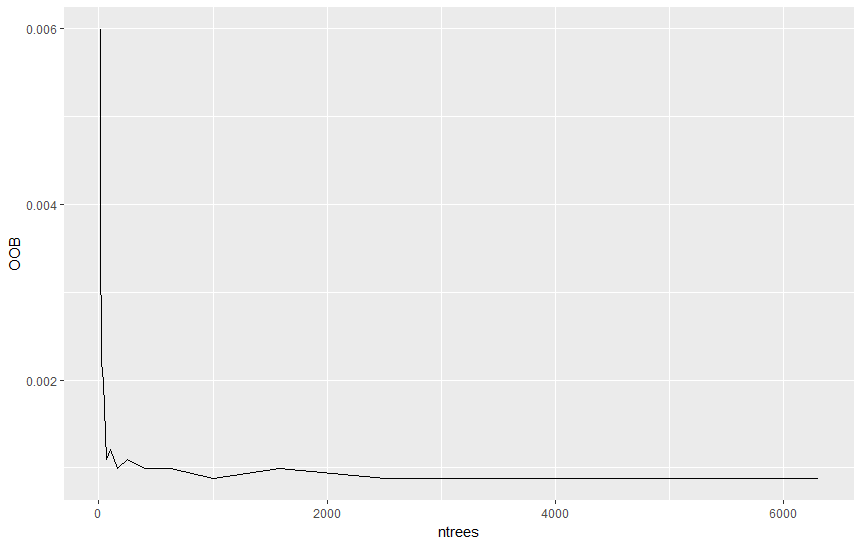
\includegraphics[scale=0.45]{ntrees.png}
	\caption{Valors de OBB per cada nombre d'arbres provat al random forest}
	\label{fig:trees}
\end{figure}

Veiem que l'error s'estabilitza a partir d'uns 2000 arbres, aproximadament. Així hem entrenat amb el nombre d'arbres que ha sortit com a millor dels que hem provat, en aquest cas ha estat 2000, i hem obtingut un error OBB del 0.1\% i un de test del 7.51\%. Creiem que la diferència entre aquests dos és deguda a que el conjunt de dades balancejat conté molt poques observacions en comparació a l'original. A més a més, el conjunt de test que ens proporciona el concurs \textit{kdd}\cite{kdd}, té moltes més observacions i tipus específics d'atacs que no existien a l'original, és per això que en aquest cas l'OOB no ha estat un bon estimador de l'error de predicció real. La taula \ref{table:random} mostra la matriu de confusió pel model obtingut. És molt més balancejat que el model que utilitzava totes les dades. Té el problema que tenen gairebé tots els models i és que el nombre de falsos negatius és bastant significatiu.

\begin{table}[H]
	\centering
	\begin{tabular}{c | c c c c c}
			& Prediction\\
		Truth\\
				& Normal & DOS & Probe & R2L & U2R \\
		\hline
		Normal	& 60147	& 39 	 & 263	 & 17 	& 125 \\
		DOS		& 6363	& 223113 & 364	 & 10  	& 3\\
		Probe	& 556	& 135	 & 3414	 & 61	&  0 \\
		R2L		& 15015	& 1		 & 44   & 901 & 228\\
		U2R		& 86	& 0		 & 80    &  10 	& 52\\	
	\end{tabular}
	\caption{Taula de contingència per el model Random Forest}
	\label{table:random}
\end{table}


\section{Selecció del model final}
Escollim les xarxes MLP com a model final degut a que els errors tant de test com de training són millors respecte als altres models amb els quals hem experimentat. A més a més podem veure que el problema no és separable amb fronteres lineals. Per tant, és lògic que obtinguem millors resultats amb els mètodes no-lineals. \\
L'error de generalització del model seleccionat és del 7.317\%. Com podem veure a la taula \ref{table:nnet_table} en general l'error està més equilibrat que en la resta de models, fet que és important donada la naturalesa de les dades.
\section{Conclusions}
\subsection{Dubtes, objectius acomplerts i objectius no acomplerts}

\begin{itemize}
    \item Hem aconseguit distingir la naturalesa de les dades i descriure-les.
    \item Hem pogut visualitzar les dades mitjançant FDA.
    \item Hem donat una solució al problema de les dades desequilibrades.
    \item Hem sabut identificar les diferents agrupacions que formen les nostres dades.
    \item Malgrat la naturalesa de les dades, obtenim uns errors d'entrenament i de generalització significativament baixos.
    \item Ens hagués agradat poder experimentar amb més models.
    \item A causa del problema de les dades desequilibrades, hem hagut de reduir moltes observacions que podrien haver estat rellevants.
    \item Degut al problema anterior hem hagut de generar dades artificials d'alguna de les classes.
    \item Ens quedem amb el dubte de saber si haguéssim pogut tractar les dades i la seva naturalesa redundant i desequilibrada per obtenir millors resultats.
    \item Tenim un nombre considerable d'atacs predits com a connexió normal, que són els pitjors en aquest domini.
\end{itemize}

\subsection{Conclusions científiques i personals}
El problema més important amb el qual ens hem hagut d'enfrontar és de tenir un conjunt de dades desequilibrades, pel que fa a la variable predictiva(main\_atack). L'hem solucionat reduint les observacions de les classes majoritàries i generant observacions sintètiques de les classes minoritàries. Com a conseqüència el conjunt de dades ha quedat molt reduït i és molt possible que hàgim perdut observacions rellevant per a la tasca de classificació. Malgrat això l'error de generalització ha empitjorat poc i l'equilibri de les dades predites ha millorat significativament.

Hem pogut posar a la pràctica alguns dels mètodes apresos a l'assignatura que coneixíem bé de forma teòrica, però no els havíem usat en un cas real. Per tant hem hagut d barallar-nos amb temps d'execució molts llargs i amb particularitats de cada algorisme que fan que aprenguem a utilitzar-los. Hem hagut de tractar unes dades reals, molt lluny de ser un exemple de joguina amb els seus problemes com la manca de normalitat de les diferents variables, el desequilibri de de les dades, el volum tant d'observacions com de l'algorisme, etc.
Ens hem pogut enfrontar amb tots aquests problemes, hem pogut trobar una solució de la majoria d'ells i d'això ens n'enduem moltes lliçons personals.

\subsection{Possibles extensions}
Una possible millora seria focalitzar els nostres esforços en les dades: entendre-les millor, tractar-les en conseqüència i d'aquesta manera obtenir millors resultats. Altres treballs existents\cite{kdd_better}, ja han tractat aquest tema i han aconseguit un conjunt de dades més net, amb menys redundància, més equilibrat etc. Nosaltres creiem que el repte d'aquest problema era poder enfrontar-nos a la dificultat de les dades i per tant no hem utilitzat aquest conjunt de dades. Com a possible extensió podríem seguir un procés similar al d'aquests treballs.

Per altra banda, podríem haver utilitzat més models de \textit{machine learning}. No ho hem fet ja sigui per manca de temps o bé perqué alguns models com els de \textit{boosting} no els hem vist a classe.
%----------------------------------------------------------------------------------------
%	BIBLIOGRAPHY
%----------------------------------------------------------------------------------------
\nocite{*}
\printbibliography

%----------------------------------------------------------------------------------------


\end{document}